\chapter{Некоторые сведения о технологиях, задействованных в разработке 2D игр}
\section{Процессы и потоки в Android OS. Управление памятью приложений}

Когда запускается компонент приложения и приложение не имеет других запущенных компонентов, Android создает новый процесс для приложения с одним потоком исполнения. По умолчанию все компоненты одного приложения запускаются в одном процессе, в потоке называемом «главный». Если компонент приложения запускается и уже существует процесс для данного приложения(какой-то компонент из приложения существует), тогда компонент запущен в этом процессе и использует его поток выполнения. Вы можете изменить данное поведение, задав разные процессы для разных компонентов вашего приложения. Кроме того вы можете добавить потоки в любой процесс.

Задать отдельный процесс для компонента можно с помощью файла манифеста. Каждый тег компонента(activity, service, receiver и provider) поддерживает атрибут android:process. Данный атрибут позволяет задать процесс, в котором будет выполняться компонент. Также вы можете задать процесс в котором будут выполняться компоненты разных приложений. Также данный атрибут поддерживается тегом application, что позволяет задать определенный процесс для всех компонентов приложения.

Android пытается поддерживать процесс приложения как можно дольше, но когда потребуются ресурсы старые процессы будут вытеснены по иерархии важности.

Существует 5 уровней иерархии важности: (процессы первого уровня из списка будут удалены последними)

\begin{itemize}
\item Процесс с которым взаимодействует пользователь(Foreground process)
К таким процессам относится например: активити с которым взаимодействует пользовать; сервис(экземпляр Service), с которым взаимодействует пользователь; сервис запущенный методом startForeground(); сервис, который выполняет один из методов своего жизненного цикла; BroadcastReceiver который выполняет метод onReceive().

\item Видимый процесс
Процесс, в котором не выполнены условия из пункта №1, но который влияет на то, что пользователь видит на экране. К примеру, вызван метод onPause() активити.

\item Сервисный процесс
Служба запущенная методом startService()

\item Фоновый процесс
Процесс выполняемый в фоновом режиме, который невиден пользователю.

\item Пустой процесс

\end{itemize}

Отмечу, что в компонентах приложения существует метод onLowMemory(), но полагаться на то, что данный метод будет вызван нельзя, также как нельзя на 100% полагаться на метод onDestroy(), поэтому логику сохранения данных или каких-либо настроек можно осуществить в методе onStop(), который(как уверяют) точно вызывается.

Когда запускается приложение, система создает «главный» поток выполнения для данного приложения, который также называется UI-потоком. Этот поток очень важен, так как именно в нем происходит отрисовка виджетов(кнопочек, списков), обработка событий вашего приложения. Система не создает отдельный поток для каждого экземпляра компонента. Все компоненты, которые запущенны в одном процессе будут созданы в потоке UI. Библиотека пользовательского интерфейса Android не является потоково-безопасной, поэтому необходимо соблюдать два важных правила:

\begin{itemize}
\item Не блокировать поток UI
\item Не обращаться к компонентам пользовательского интерфейса не из UI-потока
\end{itemize}

\underline{ AsyncTask } позволяет выполнить асинхронную работу и делать обновления пользовательского интерфейса.
Для обновления реализуйте метод onPostExecute(), а всю фоновую работу заключите в метод doInBackground(). После того, как вы реализуете свою собственную задачу, необходимо ее запустить методом execute().

Параметры передаваемые в AsyncTask:
\begin{itemize}
\item Параметры
\item Прогресс(единицы задающие ход изменения задачи)
\item Результат выполнения задачи
\end{itemize}

Отмечу пару важных моментов, которые нужно учитывать:
\begin{itemize}

\item Метод doInBackGround() выполняется в фоновом потоке, потому доступа к потоку UI внутри данного метода нет.
\item Методы onPostExecute() и onProgressUpdate() выполняются в потоке UI, потому мы можем смело обращаться к нашим компонентам UI.
\end{itemize}

Android не поддерживает swap памяти. Это означает, что любые манипуляции, связанные с памятью, например, создание новых объектов, никак не влияют на выделенную память : она постоянна в RAM. Поэтому, единственно верный способ полного освобождения памяти текущего приложения - это освободить ссылки на объекты, таким образом делая память доступной сборщику мусора. 

С целью обеспечения всех своих текущих потребностей в RAM, Android старается поделить её между между процессами. Это может быть достигнуто следующими путями :

Каждый процесс приложения ответвляется от Zygote процесса. Zygote процесс начинает работу при запуске системы и загружает общие ресурсы (например, activity themes). Для того, чтобы новый процесс приложения, система ответвляет Zygote процесс, после чего загружает и запускает код приложения в новом процессе. Это позволяет большей части страничной памяти RAM, выделенной для ресурсов, быть поделённой между всеми процессами.


\section{TCP и UDP протоколы}
TCP и UDP

Протокол UDP (User Datagram Protocol) – протокол транспортного уровня, входящий в стек протоколов TCP/IP, обеспечивающий негарантированную доставку данных без установления виртуального соединения.

Поскольку на протокол не возлагается задач по обеспечению гарантированной доставки, а лишь требуется обеспечивать связь между различными программами, то структура заголовка дейтаграммы UDP (так называется пакет протокола) выглядит достаточно просто – она включает в себя всего четыре поля. Первые два поля содержат номера UDP-портов программы-отправителя и программы-получателя. Два остальных поля в структуре заголовка дейтаграммы предназначены для управления обработкой – это общая длина дейтаграммы и контрольная сумма заголовка.

Протокол TCP (Transmission Control Protocol) является транспортным протоколом стека протоколов TCP/IP, обеспечивающим гарантированную доставку данных с установлением виртуального соединения. 

Протокол предоставляет программам, использующим его, возможность передачи непрерывного потока данных. Данные, подлежащие отправке в сеть, разбиваются на порции, каждая из которых снабжается служебной информацией, то есть формируются пакеты данных. В терминологии TCP пакет называется сегментом.

В соответствии с функциональным назначением протокола структура TCP-сегмента предполагает наличие следующих информационных полей:

\begin{itemize}
\item номер порта-отправителя и номер порта-получателя – номера портов, идентифицирующие программы, между которыми осуществляется взаимодействие;
\item поля, предназначенные для обеспечения гарантированной доставки: размер окна, номер последовательности и номер подтверждения 
\item управляющие флаги – специальные битовые поля, управляющие протоколом. 
\end{itemize}

Реализация режима гарантированной доставки
Для обеспечения гарантированной доставки протокол TCP использует механизм отправки подтверждения. С целью снижения загрузки сети протокол TCP допускает посылку одного подтверждения сразу для нескольких полученных сегментов. Объем данных, которые могут быть переданы в сеть отправителем до получения подтверждения, определяется специальным параметром протокола TCP - размером окна. Размер окна согласуется при установлении соединения между отправителем и получателем и может автоматически изменяться программными модулями протокола TCP в зависимости от состояния канала связи. Если в процессе передачи данных потери происходят достаточно часто, то размер окна уменьшается, и наоборот – окно может иметь большой размер, если высока надежность канала данных. 

Для того, чтобы данные могли быть правильно собраны получателем в нужном порядке, в заголовке TCP-сегмента присутствует информация, определяющая положение вложенных данных в общем потоке. Отправляя подтверждение, получатель указывает положение данных, которые он ожидает получить в следующем сегменте, тем самым косвенно сообщая отправителю, какой фрагмент общего потока был успешно принят. Соответствующие поля заголовка TCP-сегмента получили название номер последовательности и номер подтверждения.

Установление соединения
Перед началом передачи потока данных абоненты должны согласовать параметры передачи: размер окна и начальные номера последовательностей, относительно которых будет отсчитываться положение передаваемых в сегментах данных внутри общего потока. Очевидно, что такое согласование предполагает обмен специальными сегментами и выделение ресурсов, в частности, блоков памяти, необходимых для приема и обработки данных и подтверждений. Соответствующая последовательность действий называется установлением виртуального соединения.

\section{Netty}
Netty - это  non-blocking I/O (NIO)  клиент-серверный фреймворк предназначенный для разработки сетевых приложений на языке Java. Асинхронный событийно-ориентированный фрэймворк используемый для упрощения написания сетевых програм таких как TCP и UDP серверы. В отличии от традиционных Java-реализаций для работы с сетевыми протоколами, использующих синхронную модель передачи данных, Netty позволяет использовать асинхронную передачу, а также службы уровня операционной системы для достижения максимальной скорости передачи данных.

Для своей работы NIO использует:
\begin{itemize}
\item буферы — типы для хранения данных;
\item каналы — аналоги потоков для быстрой записи или чтения данных.
\end{itemize}


\section{Физика???}
Конечного пользователя интересует визуальное поведение игровых объектов.
Оно определяется положением тел в пространстве и времени и изучается кинематикой. Однако
кинематика не рассматривает причины возникновения движения --- этим занимается динамика. Поэтому
моделирование игровой сцены строится в следующем порядке: моделируется динамика (т.е. взаимодействие тел), на
его основе строится кинематическое описание, которое непосредственно и видит игрок. Фактически
моделирование игровой физики сводится к решению соответствующей обратной задачи механики.

%  \/ ээээ....я не знаю, что здесь написать
% спросить у меня или почитать :)
% TODO добавить абзац о различных способах аналитического моделирование одних и тех же явлений: 
% силовая динамика, законы сохранения, принцип наименьшего действия

% Обосновать необходимость численного моделирования

% \/ так же нет идеи что псиать здесь о точке и упругом теле. 
% \/ А о твёрдом теле рассказывается ниже в сответствующей подсекции
% имеется ввиду важность с точки зрения самой физики этих моделей
% TODO добавить абзац о материальной точке, абсолютно твердом теле и упругом теле

\subsection{Кинематическое описание}
\subsubsection{Материальная точка}
Положение тела в пространстве в любой момент времени задается функцией радиус вектора от
времени, получившей исторически название уравнение движения:
\begin{equation}
 \mathbf{r}=\mathbf{r}(t).
\end{equation}

Непосредственный вид уравнения движения может быть задан лишь в ограниченном числе 
тривиальных случаев. В реальных же задачах мы можем получить на основе динамики 
дифференциальное уравнение (или систему в случае многих тел), решением которого
будет искомое уравнение движения.
\begin{equation}
 \ddot{\mathbf{r}}=f(t, \mathbf{r}(t), \dot{\mathbf{r}}(t)).
\end{equation}

Первой и второй производной является скорость и ускорение соответственно.
Так как механическое состояние системы полностью характеризуется заданием координат
и скоростей \cite[10]{Landau1}, то возможны уравнения не выше второго порядка. 
В данном случае, скорость и ускорение --- величины векторные, поскольку они имеют величину и направление.

\subsubsection{Твердое тело}
Лишь некоторые тела могут быть промоделированы заданием лишь одного положения в пространстве 
(например, материальная точка), большинство тел имеет форму и по разному ведут себя в зависимости
от ориентации в пространстве. Существует несколько способов задания ориентации тела в трехмерном
пространстве. Изменение положения тела в пространстве характеризуются двумя псевдовекторами ---
угловой скоростью и угловым ускорением.
\subsubsection{Углы Эйлера}
% \/ попытался
%TODO здесь толком описать углы Эйлера (желательно с картинками) и проблему шарнирного замка
Углы Эйлера --- углы, описывающие поворот абсолютно твердого тела в трехмерном евклидовом пространстве.

Углы Эйлера определяют три поворота системы\cite[79]{Berezkin}, которые позволяют привести любое положение системы к текущему.
Обозначим начальную систему координат как ($x$, $y$, $z$), конечную как ($X$, $Y$, $Z$).
Пересечение координатных плоскостей $xy$ и $XY$ называется линией узлов $N$.
\begin{itemize}
  \item Угол $\alpha$ между осью $x$ и линией узлов --- угол прецессии.
  \item Угол $\beta$ между осями $z$ и $Z$ --- угол нутации.
  \item Угол $\gamma$ между осью $X$ и линией узлов --- угол собственного вращения.
\end{itemize}
  
Повороты системы на эти углы называются прецессия, нутация и поворот на собственный угол (вращение).
Такие повороты некоммутативны и конечное положение системы зависит от порядка, в котором совершаются повороты. 

\begin{figure}[ht!]
\begin{center}
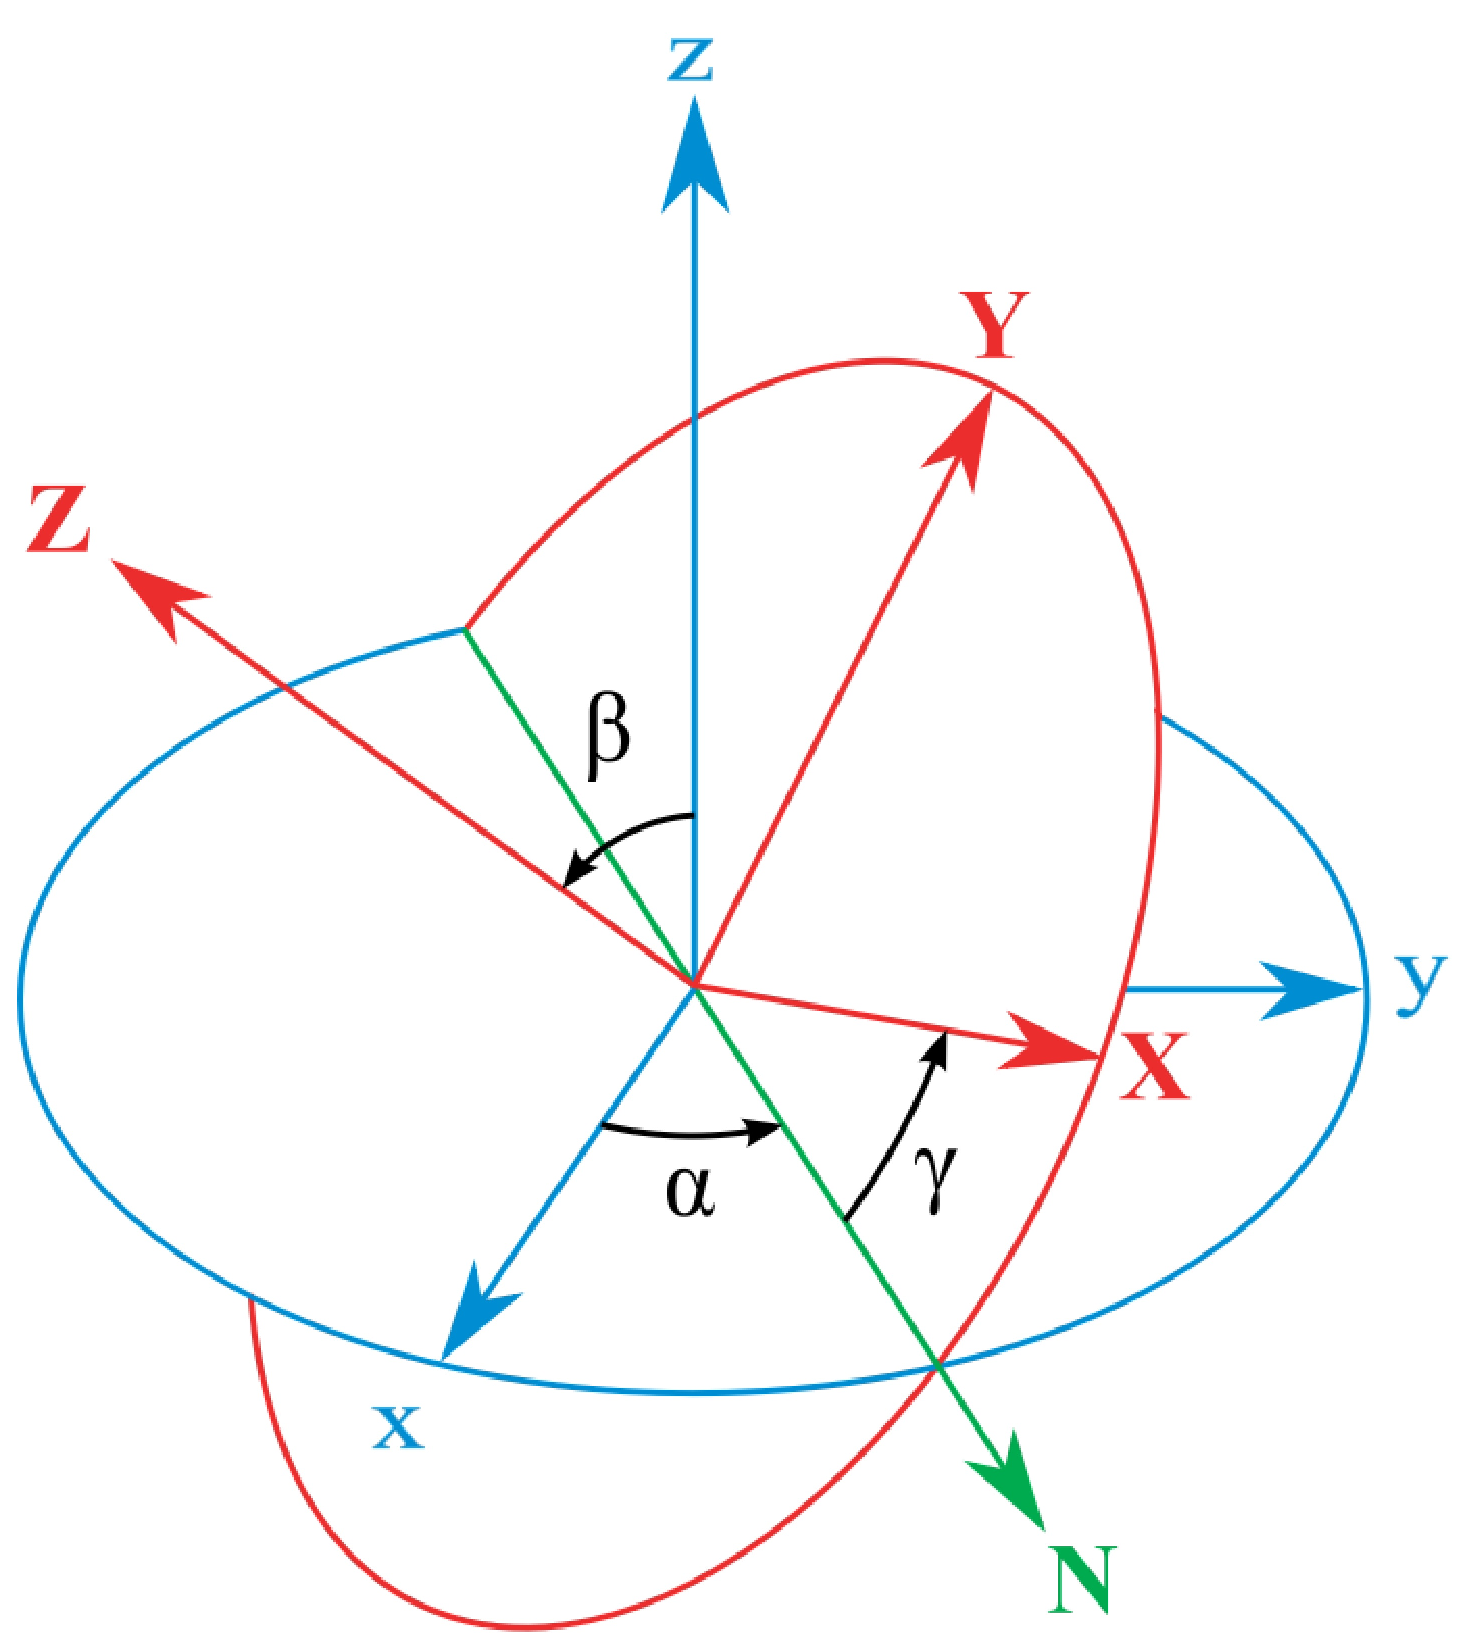
\includegraphics[scale=0.25]{./Rigidbody/Eulerangles.eps}  \\
\caption{Углы Эйлера}\label{Eulerangles}
\end{center}
\end{figure}

\subsubsection{Матрица поворота}
% \/  ...попытался
%TODO описать матрицу поворота
Матрицей поворота (или матрицей направляющих косинусов) называется ортогональная матрица,
которая используется для выполнения собственного ортогонального преобразования в евклидовом пространстве.
При умножении любого вектора на матрицу поворота длина вектора сохраняется. Определитель матрицы поворота равен единице.
Обычно считают, что, в отличие от матрицы перехода при повороте системы координат (базиса),
при умножении на матрицу поворота вектора-столбца координаты вектора преобразуются в соответствии с поворотом
самого вектора (а не поворотом координатных осей; то есть при этом координаты повернутого вектора получаются в той же,
неподвижной системе координат). Однако отличие той и другой матрицы лишь в знаке угла поворота,
и одна может быть получена из другой заменой угла поворота на противоположный; та и другая взаимно обратны и могут быть получены
друг из друга транспонированием.

Любое вращение в трехмерном пространстве может быть представлено как композиция поворотов вокруг
трех ортогональных осей (например, вокруг осей декартовых координат).
Этой композиции соответствует матрица, равная произведению соответствующих трех матриц поворота.
Матрицами вращения вокруг оси декартовой системы координат на угол $\alpha$ в трехмерном пространстве являются:
\begin{itemize}
  \item Вращение вокруг оси $x$:
  \begin{equation}
    \mathrm{M}_x(\alpha) = 
    \begin{pmatrix} 
      1 & 0          & 0 \\
      0 & \cos\alpha & -\sin\alpha \\
      0 & \sin\alpha & \cos\alpha
    \end{pmatrix},
  \end{equation}
  
  \item Вращение вокруг оси $y$:
  \begin{equation}  
    \mathrm{M}_y(\alpha) = 
    \begin{pmatrix} 
      \cos\alpha  & 0 & \sin\alpha \\
      0           & 1 & 0           \\
      -\sin\alpha & 0 & \cos\alpha
    \end{pmatrix},
  \end{equation}
  \item Вращение вокруг оси $z$:
  \begin{equation}
    \mathrm{M}_z(\alpha) = 
    \begin{pmatrix} 
      \cos\alpha & -\sin\alpha & 0 \\
      \sin\alpha & \cos\alpha  & 0 \\
      0          & 0           & 1
    \end{pmatrix}.
  \end{equation}
\end{itemize}
Во всех примерах приведены матрица поворота от результирующей системы координат к исходной.
  
\subsubsection{Кватернион}
% \/  ...попытался
%TODO описать кватернион и его связь с поворотом и угловой скоростью

Кватернионы\cite[11]{Kantor} предоставляют удобное математическое обозначение положения и вращения объектов в пространстве.
В сравнении с углами Эйлера, кватернионы позволяют проще комбинировать вращения\cite[17]{Altmann}, а также избежать проблемы,
связанной с невозможностью поворота вокруг оси, независимо от совершенного вращения по другим осям.
В сравнении с матрицами они обладают большей вычислительной устойчивостью и могут быть более эффективными.
Кватернионы нашли свое применение в компьютерной графике, робототехнике, навигации, молекулярной динамике.

Кватернион выгодно использовать в компьютерных вычислениях, так как представление кватерниона требует
лишь 4 компоненты, против 9 компонент (3 вектора по 3 компоненты) у углов Эйлера и 9 компонент у матрицы поворота.

\subsection{Динамическое описание}
Согласно силовой модели механики равнодействующая сил приложенных к телу вызывает ускорение (второй закон Ньютона)
\begin{equation}
 \mathbf{a}=\frac{\sum\limits_{i=1}^n{\mathbf{F}_i}}{m}.
\end{equation}
Всего существует только четыре природы силовых взаимодействий: гравитационная, электромагнитная, сильная и слабая.
Последние две проявляют себя только на микроуровне, поэтому их нет необходимости рассматривать в задачах
игровой физики. Гравитационная природа представлена полем тяготения, которое является консервативным. 
Все остальные силы являются проявлением взаимодействий электромагнитной природы на микро и макроуровне.
Однако оказывается весьма неудобным при рассмотрении макроявлений использовать электромагнитные силы на микроуровне,
поэтому вводятся макрообощения характеризующее соответствующее явление в целом, например, закон Кулона
для трения или закон Гука для упругости.

Во многих случаях даже такое макроописание является слишком подробным и сложно реализуемым на компьютере,
поэтому часто моделируют только абсолютно твердые тела, для взаимодействия которых выполняется закон 
сохранения импульса.
\subsubsection{Динамика вращательного движения}
Для вращательного движения тела можно ввести ряд характеристик
являющимися аналогами уже рассмотренных для поступательного движения.
Радиус вектору $ \mathbf{r} $ соответствует кватернион $q$ или матрица вращения $\mathrm{R}$,
скорости $\mathbf{v}$ --- угловая скорость $\boldsymbol{\omega}$ направленная вдоль оси вращения,
ускорению $\mathbf{a}$ --- $\boldsymbol{\alpha}$ угловое ускорение.
Вызванное силой вращение зависит не только от силы, но и от положения точки приложения силы
по отношению к мгновенному центру вращения, величина аналогичная силе носит название момента силы:
\begin{equation}
 \mathbf{M} = \mathbf{r}\times{\mathbf{F}}, 
\end{equation}
она также как и сила является аддитивной величиной.

Мера отклика на момент силы зависит не только от массы тела, но и от геометрии распределения
масс в теле. Данная величина получила название момента инерции тела:
\begin{equation}
 J=\int\limits_{V} \rho r^2\mathrm{d}V.
\end{equation}

В общем случае момент инерции зависит от направления оси вращения и поэтому является тензорной
величиной $\mathrm{J}$ (фактически двухмерной матрицей \begin{math}3\times3\end{math}), компоненты которого могут
быть выражены как:
\begin{equation}
 \mathrm{J}_{ij} = \int\limits_{V} (\delta_{ij}r^2 - \mathbf{r}_i \mathbf{r}_j) \rho \mathrm{d}V,
\end{equation}
где $\delta_{ij}$ символ Кронекера, а $\mathbf{r}$ радиус-вектор из центра вращения к точке интегрирования.
Тензор инерции всегда является положительно определенным и может быть приведен к диагональному виду. Момент
инерции относительно произвольно расположенной оси вращения может быть выражен через момент инерции параллельной
оси вращения проходящей через центр масс по теореме Гюйгенса--Штейнера:
\begin{equation}
 J=J_C+md^2.
\end{equation}

%TODO Дать формулу связывающую момент силы, момент инерции и угловое ускорение в случае, 
% когда момент инерции является тензорной величиной. (я пока нашёл лишь через кососимметричные матрицы) 
% также в обязательном порядке дать корректные формулировки связи кватерниона и угловой скорости
%\begin{equation}
%q = \frac{1}{2}q_0\omega{\delta{t}} 
%\end{equation}

% Возможно нужно что-то ещё, но собственно это резюме этой части
Таким образом, динамическое тело может быть описано
следующими минимальными характеристиками:
\begin{itemize}
  \item масса (скаляр)
  \item позиция (вектор)
  \item скорость (вектор)
  \item ускорение (вектор) %???
  \item сумма сил (вектор) %???
  \item момент инерции (матрица)
  \item поворот (кватернион)
  \item угловая скорость (вектор)
  \item угловое ускорение (вектор) %???
  \item сумма моментов сил (вектор) %???
\end{itemize}
